\documentclass[tikz, border=3.14mm]{standalone}
\usepackage{pgfplots}
\pgfplotsset{compat=1.18}
\usepgfplotslibrary{groupplots}

\begin{document}
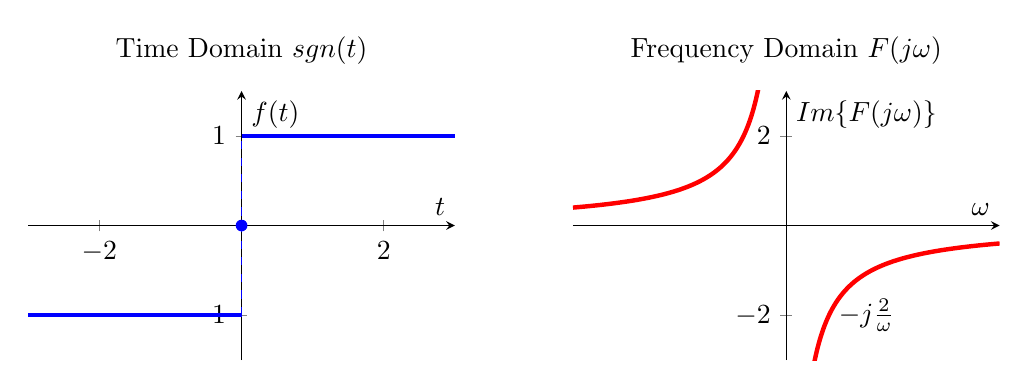
\begin{tikzpicture}
    \begin{groupplot}[
        group style={group size=2 by 1, horizontal sep=1.5cm},
        axis lines = middle,
        width = 7cm, height = 5cm,
        ymin = -1.5, ymax = 1.5,
        grid=none,
        xlabel = {$t$},
        ylabel = {$f(t)$}
    ]
        % Time Domain Signum
        \nextgroupplot[
            title = {Time Domain $sgn(t)$},
            xmin = -3, xmax = 3,
            ytick = {-1, 1}
        ]
        \draw[ultra thick, blue] (-3,-1) -- (0,-1);
        \draw[ultra thick, blue] (0,1) -- (3,1);
        \draw[blue, dashed] (0,-1) -- (0,1);
        \node[circle, fill=blue, inner sep=1.5pt] at (0,0) {};

        % Frequency Domain Signum (Imaginary)
        \nextgroupplot[
            title = {Frequency Domain $F(j\omega)$},
            xlabel = {$\omega$},
            ylabel = {$Im\{F(j\omega)\}$},
            xmin = -5, xmax = 5,
            ymin = -3, ymax = 3,
            samples = 200,
            xtick = \empty,
            clip = true
        ]
        \addplot[ultra thick, red, domain=-5:-0.1] {-2/x};
        \addplot[ultra thick, red, domain=0.1:5] {-2/x};
        \node[anchor=west] at (axis cs:1, -2) {$-j\frac{2}{\omega}$};

    \end{groupplot}
\end{tikzpicture}
\end{document}
